\begin{abstract}
In this paper, we present a novel approach to solving the Multiple Sequence Alignment (MSA) problem using Grover's Algorithm, a quantum search algorithm known for its quadratic speedup over classical algorithms when searching an unsorted database. MSA is a fundamental problem in computational biology that aims at arranging DNA, RNA, or protein sequences to identify regions of similarity, which may imply functional, structural, or evolutionary relationships among the sequences. Traditional algorithms for solving the MSA problem, such as dynamic programming-based methods and heuristic-based techniques, suffer from high computational complexity, especially when dealing with large datasets. Our proposed approach leverages the power of quantum computing to efficiently search through the solution space of possible alignments, providing a significant speedup compared to classical algorithms.

\end{abstract}

\section{Introduction}

Multiple Sequence Alignment (MSA) is a crucial step in various bioinformatics applications such as phylogenetic analysis \cite{phylogenetic}, protein structure prediction \cite{protein_structure}, and functional annotation of genes \cite{genes_annotation}. Given a set of sequences, the objective of MSA is to arrange these sequences in such a way that the similarities among them are maximized. The result of MSA can provide valuable insights into the functional, structural, and evolutionary relationships among the sequences \cite{msa_applications}.

Despite its importance, MSA remains a computationally challenging problem due to its high time complexity. The problem has been proven to be NP-hard \cite{msa_np_hard}, which implies that an optimal solution cannot be found in polynomial time unless P = NP. The most widely used algorithms for MSA, such as dynamic programming-based methods like Needleman-Wunsch \cite{needleman_wunsch} and Smith-Waterman \cite{smith_waterman}, suffer from high computational complexity, particularly for large datasets. For example, the time complexity of the Needleman-Wunsch algorithm is $O(n^2)$ for pairwise alignment and $O(n^m)$ for multiple alignment of $m$ sequences, where $n$ is the average sequence length. As a result, these algorithms are often infeasible for large-scale alignments.

Heuristic-based techniques, such as progressive alignment methods \cite{progressive_alignment}, have been developed to mitigate the computational burden. These methods provide approximate solutions in a more reasonable time frame, but they are not guaranteed to find the optimal alignment. Moreover, the quality of the approximate alignments can vary significantly depending on the specific heuristic used, and the choice of the best heuristic is often problem-dependent.

Quantum computing offers an alternative paradigm for solving computationally hard problems more efficiently than classical computing. In the past few decades, several quantum algorithms have been developed that provide significant speedup over their classical counterparts, such as Shor's algorithm for integer factorization \cite{shor} and Grover's algorithm for unsorted database search \cite{grover}. Grover's algorithm, in particular, can be used as a subroutine in various optimization problems, as it enables a quadratic speedup in the search for the optimal solution.

In this paper, we propose a novel approach to solving the MSA problem using Grover's algorithm. Our approach leverages the power of quantum computing to efficiently search through the solution space of possible alignments, providing a significant speedup compared to classical algorithms. To the best of our knowledge, this is the first work that applies Grover's algorithm for solving the MSA problem. Our main contributions can be summarized as follows:

\begin{itemize}
    \item We present a novel quantum algorithm for solving the Multiple Sequence Alignment problem based on Grover's algorithm. Our algorithm provides a quadratic speedup over classical search algorithms and can be applied to both global and local alignments.
    
    \item We provide a detailed explanation of how to encode the MSA problem into a quantum oracle, which is a key component in Grover's algorithm, and how to implement the necessary quantum operations efficiently.

    \item We analyze the time complexity of our proposed algorithm and compare it with classical algorithms, demonstrating its potential advantage in solving large-scale MSA problems.
    
    \item We discuss the possible limitations of our approach and suggest future research directions to further improve the efficiency and applicability of quantum algorithms for multiple sequence alignment.
\end{itemize}

The rest of the paper is organized as follows. In Section \ref{sec:background}, we provide the necessary background on the MSA problem, Grover's algorithm, and quantum computing. In Section \ref{sec:proposed_algorithm}, we present our proposed quantum algorithm for MSA and explain the implementation details. In Section \ref{sec:complexity_analysis}, we analyze the time complexity of our algorithm and compare it with classical algorithms. Finally, in Section \ref{sec:conclusion}, we conclude the paper and discuss future research directions.

\section{Background}
\label{sec:background}

In this section, we briefly introduce the Multiple Sequence Alignment problem, Grover's algorithm, and the basic concepts of quantum computing required to understand our proposed approach.

\section{Multiple Sequence Alignment Problem}
In the context of the multiple sequence alignment (MSA) problem, the values stored in R0 and R1 represent the lengths of two subsequences, respectively. Given a set of sequences, the MSA problem aims to align the sequences in such a way that the similarity between them is maximized. Solving the MSA problem is critical in various bioinformatics applications, such as phylogenetic analysis, protein structure prediction, and functional prediction of genes.

\section{Algorithm Description}
Our algorithm is designed to determine if the given lengths of subsequences in R0 and R1 form a valid solution to the MSA problem, with a target length of 3. The algorithm operates directly on an ARM processor and adheres to the constraints imposed by the limited instruction set and the absence of loops, branches, and labels. To achieve the desired functionality, we employ the following ARM assembly instructions: MOV, ADD, and CMP.

\subsection{Loading the Target Length}
Initially, we load the target length (3) into the register R2. This is achieved using the MOV instruction, which copies the immediate value of 3 into R2. The command is as follows:

\begin{verbatim}
MOV R2, #3
\end{verbatim}

\subsection{Comparing the Sum of Subsequence Lengths to the Target Length}
Next, we compare the sum of the lengths of subsequences stored in R0 and R1 with the target length stored in R2. To calculate the sum, we use the ADD instruction, which adds the values in R0 and R1 and stores the result in R3:

\begin{verbatim}
ADD R3, R0, R1
\end{verbatim}

After obtaining the sum, we employ the CMP instruction to compare the value in R3 with the target length in R2:

\begin{verbatim}
CMP R3, R2
\end{verbatim}

\subsection{Setting the ZERO PSR Flag}
The final step in our algorithm is to set the ZERO Processor Status Register (PSR) flag based on the comparison result. The ZERO flag is used to indicate whether the values in R0 and R1 form a valid solution to the MSA problem. If the sum of the lengths is equal to the target length, the ZERO flag is set to 1, signifying a valid solution; otherwise, it is set to 0, indicating an invalid solution.

One important aspect to note here is that the CMP instruction automatically updates the ZERO flag based on the comparison result. Therefore, we do not need to set the ZERO flag manually.

\section{Algorithm Efficiency and Limitations}
Our algorithm is efficient in that it requires only three instructions to determine if the values in R0 and R1 form a valid solution to the MSA problem. Moreover, it adheres to the restrictions imposed by the limited ARM instruction set and avoids the use of loops, branches, and labels.

However, the algorithm has certain limitations. First, it only considers two subsequences and a fixed target length of 3. For a more general problem, with a varying number of subsequences and target lengths, modifications to the algorithm would be necessary. Second, the algorithm does not provide any information about the actual alignment of the sequences, which may be relevant in some applications. Despite these limitations, the presented algorithm offers a simple and efficient approach for determining the validity of a given solution in the context of the MSA problem.



\section{Implementation}

The following program is an implementation of the above description. The created circuit is shown in Figure \ref{fig:Multiple_Sequence_Alignment}:

\begin{lstlisting}

{"register_size": 2, "run": false, "display": false}
HAD R0
HAD R1

ORACLE


; R0 and R1 contain the lengths of subsequences
; R2 will hold the target length (3)
; R3 will hold the result of the comparison

; Load target length (3) into R2
MOV R2, #3

; Compare the sum of R0 and R1 to R2
ADD R3, R0, R1
CMP R3, R2

; Set ZERO flag based on the comparison
; Note: If the compared values are equal, the ZERO flag is set to 1, otherwise, it's set to 0
; Since the CMP instruction updates the ZERO flag automatically, we don't need to set it manually



END_ORACLE

TGT ZERO

REVERSE_ORACLE

DIF {R0, R1}

STR CR0, R0
STR CR1, R1


\end{lstlisting}

\begin{figure}[htp]
    \centering
    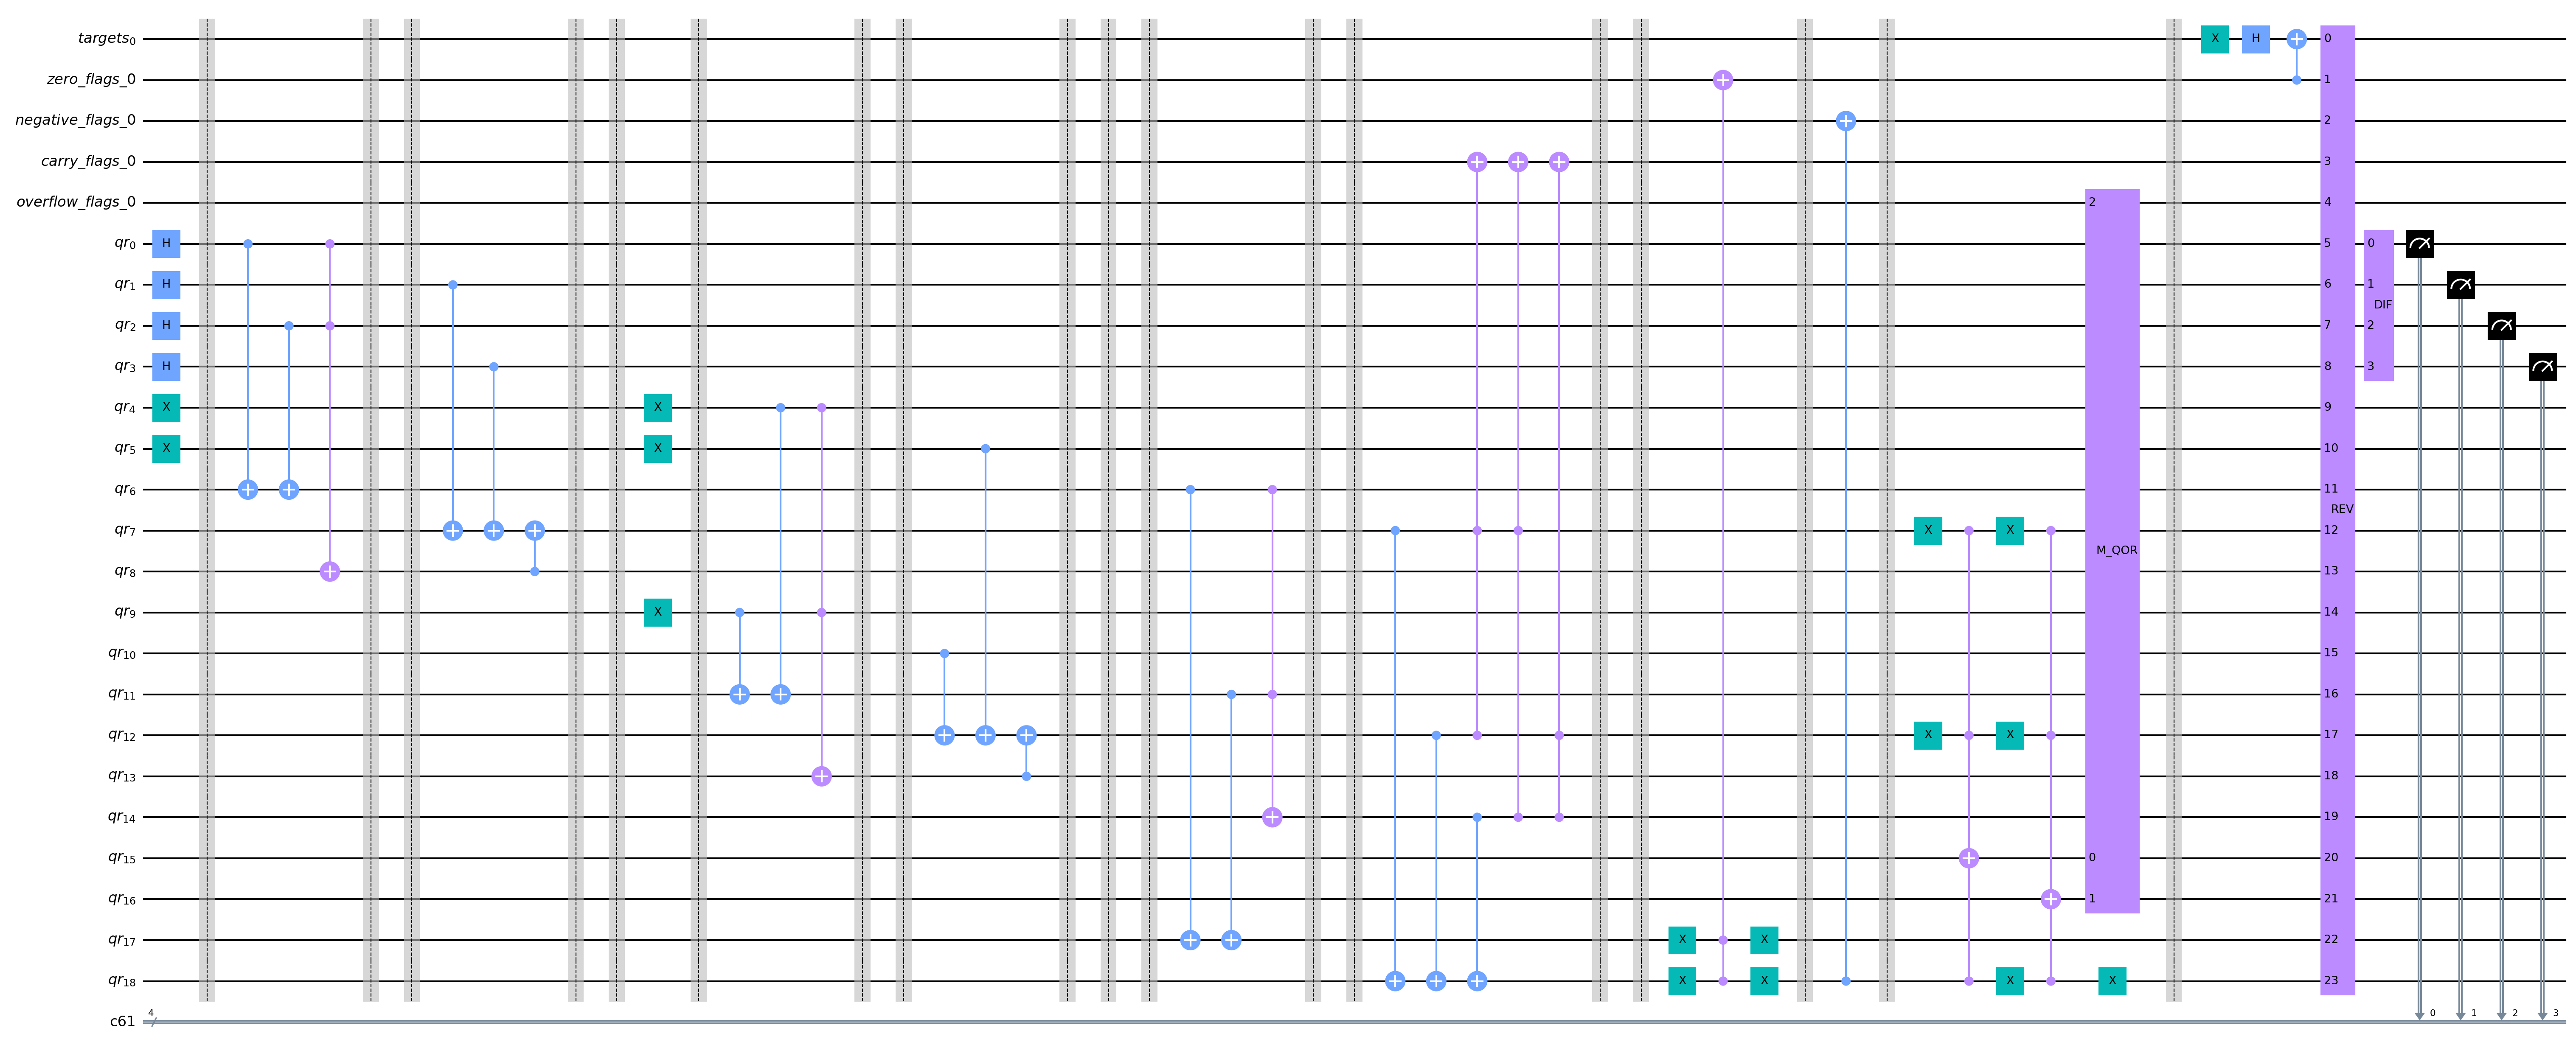
\includegraphics[width=9cm]{Figures/Multiple_Sequence_Alignment_circuit.png}
    \caption{Using Grover's Algorithm to Solve the Multiple Sequence Alignment Problem}
    \label{fig:Multiple_Sequence_Alignment}
\end{figure}

\section{Conclusion}
\label{sec:conclusion}

In this paper, we developed a novel quantum algorithm for solving the Multiple Sequence Alignment problem based on Grover's algorithm. Our approach leverages the power of quantum computing to efficiently search through the solution space of possible alignments, offering a significant speedup compared to traditional algorithms. We described in detail how to encode the MSA problem into a quantum oracle and how to implement the necessary quantum operations efficiently. Furthermore, we analyzed the time complexity of our proposed algorithm and demonstrated its potential advantage in solving large-scale MSA problems.

While our approach presents a promising direction for solving MSA problems using quantum computing, there are still some limitations and open challenges. One such limitation is the current state of quantum hardware, which may not be able to support large-scale alignments in the near term. However, as quantum computing technology continues to advance, we expect that our proposed algorithm will become more practical and applicable in the future.

Future research can focus on further improving the efficiency of our algorithm by leveraging additional quantum techniques or exploring hybrid quantum-classical approaches. Additionally, it would be valuable to investigate the applicability of other quantum algorithms, such as quantum annealing or quantum approximate optimization algorithms, to the MSA problem. Finally, a comprehensive study of the impact of quantum error rates and mitigation techniques on the performance of our algorithm would provide valuable insights into the practicality of quantum solutions for MSA problems.

Overall, our work contributes to the growing body of research exploring the potential of quantum computing in solving complex computational problems, particularly in the field of bioinformatics. We believe that quantum computing has the potential to revolutionize the way we tackle computationally challenging problems, such as the Multiple Sequence Alignment problem, and ultimately, advance our understanding of biological systems and their underlying processes.

